% mnras_template.tex 
%
% LaTeX template for creating an MNRAS paper
%
% v3.0 released 14 May 2015
% (version numbers match those of mnras.cls)
%
% Copyright (C) Royal Astronomical Society 2015
% Authors:
% Keith T. Smith (Royal Astronomical Society)

% Change log
%
% v3.0 May 2015
%    Renamed to match the new package name
%    Version number matches mnras.cls
%    A few minor tweaks to wording
% v1.0 September 2013
%    Beta testing only - never publicly released
%    First version: a simple (ish) template for creating an MNRAS paper

%%%%%%%%%%%%%%%%%%%%%%%%%%%%%%%%%%%%%%%%%%%%%%%%%%
% Basic setup. Most papers should leave these options alone.
%\documentclass[fleqn,usenatbib]{mnras}
\documentclass[12pt]{emulateapj}


% MNRAS is set in Times font. If you don't have this installed (most LaTeX
% installations will be fine) or prefer the old Computer Modern fonts, comment
% out the following line
%\usepackage{newtxtext,newtxmath}
% Depending on your LaTeX fonts installation, you might get better results with one of these:
%\usepackage{mathptmx}
%\usepackage{txfonts}

% Use vector fonts, so it zooms properly in on-screen viewing software
% Don't change these lines unless you know what you are doing
\usepackage{yfonts}
\usepackage[T1]{fontenc}
\usepackage{ae,aecompl}

%%%%% AUTHORS - PLACE YOUR OWN PACKAGES HERE %%%%%

% Only include extra packages if you really need them. Common packages are:
\usepackage{graphicx}	% Including figure files
\usepackage{amsmath}	% Advanced maths commands
\usepackage{amssymb}	% Extra maths symbols

%\usepackage{url}
\usepackage{microtype}
%\usepackage{rotating}
\usepackage{booktabs}
\usepackage{threeparttable}
\usepackage{tabularx}
\usepackage{xspace}

\usepackage{hyperref}


%%%%%%%%%%%%%%%%%%%%%%%%%%%%%%%%%%%%%%%%%%%%%%%%%%

%%%%% AUTHORS - PLACE YOUR OWN COMMANDS HERE %%%%%

% Please keep new commands to a minimum, and use \newcommand not \def to avoid
% overwriting existing commands. Example:
%\newcommand{\pcm}{\,cm$^{-2}$}	% per cm-squared
\newcommand{\project}[1]{\textsl{#1}}
\newcommand{\nustar}{\project{NuSTAR}\xspace}
\newcommand{\fermi}{\project{Fermi}\xspace}
\newcommand{\rxte}{\project{RXTE}\xspace}
\newcommand{\xmm}{\project{XMM-Newton}\xspace}
\newcommand{\rosat}{\project{ROSAT}\xspace}
\newcommand{\swift}{\project{Swift}\xspace}
\newcommand{\astrosat}{\project{Astrosat}\xspace}
\newcommand{\ixpe}{\project{IXPE}\xspace}
\newcommand{\nicer}{\project{NICER}\xspace}

\newcommand{\given}{\ensuremath{\,|\,}}
\newcommand{\dd}{\ensuremath{\mathrm{d}}}
\newcommand{\counts}{\ensuremath{y}}
\newcommand{\pars}{\ensuremath{\theta}}
\newcommand{\mean}{\ensuremath{\lambda}}
\newcommand{\likelihood}{\ensuremath{{\mathcal L}}}
\newcommand{\Poisson}{\ensuremath{{\mathcal P}}}
\newcommand{\Uniform}{\ensuremath{{\mathcal U}}}

\newcommand{\Normal}{\ensuremath{{\mathcal N}}}
\newcommand{\bg}{\ensuremath{\mathrm{bg}}}
\newcommand{\word}{\ensuremath{\phi}}

%%%%%%%%%%%%%%%%%%%%%%%%%%%%%%%%%%%%%%%%%%%%%%%%%%

%%%%%%%%%%%%%%%%%%% TITLE PAGE %%%%%%%%%%%%%%%%%%%

\begin{document}

% Title of the paper, and the short title which is used in the headers.
% Keep the title short and informative.
\title[On The Statistical Properties of Cospectra]{On The Statistical Properties of Cospectra}

% The list of authors, and the short list which is used in the headers.
% If you need two or more lines of authors, add an extra line using \newauthor
\author{D.~Huppenkothen\altaffilmark{1,2} and M.~Bachetti\altaffilmark{3}}

\altaffiltext{1}{Center for Data Science, New York University, 65 5h Avenue, 7th Floor, New York, NY 10003}
\altaffiltext{2}{Center for Cosmology and Particle Physics, Department of Physics, New York University, 4 Washington Place, New York, NY 10003, USA}
\altaffiltext{3}{INAF-Osservatorio Astronomico di Cagliari, via della Scienza 5, I-09047 Selargius (CA), Italy}


\begin{abstract}
In recent years, the cross spectrum has received considerable attention as a means of characterising the variability of astronomical sources as a function of wavelength. While much has been written about the statistics of time and phase lags, the cospectrum has only recently been understood as means of mitigating instrumental effects dependent on temporal frequency in astronomical detectors, as well as a method of characterizing the coherent variability in two  wavelength ranges on different time scales. In this paper, we lay out the statistical foundations of the cospectrum, starting with the simplest case of detecting a periodic signal in the presence of white noise. This case is especially relevant for detecting faint X-ray pulsars in detectors heavily affected by instrumental effects, including \nustar, \astrosat\ and \ixpe. We show that the statistical distributions of both single and averaged cospectra differ considerably from those for standard power spectra. While a single cospectrum follows a Laplace distribution exactly, averaged cospectra are approximated by a Gaussian distribution only for more than $\sim\!\! 30$ averaged segments, dependent on the number of trials. We provide an instructive example of a quasi-periodic oscillation in \nustar\ and show that applying standard power spectral statistics leads to underestimated tail probabilities for period detection.

\end{abstract}

% These dates will be filled out by the publisher
%\date{Accepted XXX. Received YYY; in original form ZZZ}

% Enter the current year, for the copyright statements etc.
%\pubyear{2017}

% Don't change these lines

% Abstract of the paper

% Select between one and six entries from the list of approved keywords.
% Don't make up new ones.
%\begin{keywords}
%X-rays:binaries -- X-rays:individual -- stars:black holes -- methods:data analysis -- methods:statistical
%\end{keywords}

%%%%%%%%%%%%%%%%%%%%%%%%%%%%%%%%%%%%%%%%%%%%%%%%%%

%%%%%%%%%%%%%%%%% BODY OF PAPER %%%%%%%%%%%%%%%%%%

\section{Introduction}

Time series analysis is one of the primary ways to understand the physical properties of astronomical object in our universe, from exoplanets and stars to black holes and Active Galactic Nuclei (AGN). 
Fourier analysis, especially through the periodogram\footnote{We distinguish in this paper between the \textit{power spectrum}, which describes the process at the source generating variable time series, and the \textit{periodogram}, which denotes a realization of said power spectrum, i.e.\ the time series we actually observe.}, has long been used to find periodic and quasi-periodic signals as well as characterize the stationary stochastic processes often present in accreting systems. 
While in principle, the statistics of the periodogram is well understood and characterized in the literature \citep[e.g.][]{vanderklis1989}, the periodogram is often subject to instrumental effects like dead time that change its statistical properties and thus make statistical inference difficult in practice \citep[e.g.][]{Zhang+95}.

In the past years, the field of \textit{spectral timing} has enjoyed significant success by making it possible to combine both temporal and spectral information in a single model. Within this framework, the complex cross spectrum---defined as the Fourier transform of one time series with the complex conjugate of the Fourier transform of a second time series--holds a central position. The cross spectrum is commonly used to compute phase lags, which are easily converted to time lags and are central for understanding e.g.\ reverberation mapping in accreting black holes \citep[see][for a recent review]{uttley2014}. 

The real part of the cross spectrum, also named \textit{cospectrum}, has gained less attention, but can be just as useful. It has long been used to study gravity waves in the Earth's atmosphere \citep[e.g.][]{john2016}, models of the Martian atmosphere \citep[e.g.][]{wang2016}, the solar heliosphere \citep[e.g.][]{vigeesh2017}, surface elevation of arctic sea ice \citep[e.g.][]{ardhuin2016} and drifting snow \citep[e.g.][]{paterna2016} as well as surface gravity waves in beaches \citep[e.g.][]{fiedler2015} and eddy heat flux in the Earth's troposphere \citep[e.g.][]{wang2015,zurita-gotor2017}.
Within astronomy, it has recently been recognized as one approach to mitigate instrumental effects by making use of the independent detectors present in some telescopes. Where in standard analysis, light curves of multiple detectors are summed before Fourier transforming the summed light curve, it is possible to instead Fourier-transform the signal of two independent detectors. 
The resulting powers will be less affected by an instrumental effect called dead time (see details in \citealt{Bachetti+15}), which leads to frequency-dependent changes in the mean and variance of the statistical distributions governing the periodogram. This is relevant for current X-ray detectors such as \nustar\ and \astrosat, but will also be relevant to future missions with multiple detectors like \ixpe. This approach has recently been used in \nustar\ studies of millisecond pulsars \citep{ferrigno2017}, Ultraluminous X-ray Sources \citep{bachetti2016} and X-ray binaries \citep{barriere2015,zoghbi2016,ingram2016,huppenkothen2017,stiele2017}.
Similarly, the cospectrum of two time series taken with the same instrument, but in different wavelength ranges, can be used to characterize the coherent variability in both time series as a function of frequency.

While much has been written on the subject of the statistics of cross spectra and time lags \citep[e.g.][]{epitropakis2016}, the derivation of cospectral statistics is notably absent from the astronomy literature, and most publications assume that either the $\chi^2_2$ distribution used for standard periodograms or a Gaussian distribution for averaged spectra is appropriate. That these assumptions are valid has not been shown until now. 

In this paper, we lay out the basic statistical distributions for detecting periodic and narrow quasi-periodic signals in the presence of detector noise (e.g.\ photon counting statistics) for both single and averaged cospectra. We show below that unlike for the periodogram, the statistical distribution for a single cospectrum reduces to a Laplace distribution, while the distribution for averaged cospectra is considerably more complex. We also find that for averaged cospectra consisting of more than $\sim$30 averaged individual segments, the assumption of a Gaussian distribution is indeed appropriate for single-trial tail probabilities and reduces computation overhead. However, for averaged cospectra of fewer segments, more stringent significance thresholds or large numbers of trials, the statistical distribution--and hence the derived $p$-values used for period detection--deviate significantly from a Gaussian distribution.

The paper is laid out as follows. In Section \ref{sec:single_cospectrum}, we derive the PDF of a single cospectrum, and show associated simulations and detection thresholds for period detection in Section \ref{sec:detectionthresholds}. Section \ref{sec:averaged_cospectra} extends the derivation to the common case where the cospectra of several time series are averaged. We show that the statistical distribution indeed changes from a Laplace distribution once multiple cospectra are averaged and becomes consecutively more Gaussian as a larger number of cospectra are included in the average in Section \ref{sec:averaged_detthres}. Finally, Section \ref{sec:nustarqpo} presents a real-world example using simulated \nustar\ data of a quasi-periodic oscillation (QPO) as commonly found in accreting neutron star X-ray binaries. We end in Section \ref{sec:discussion} with a short discussion and conclusion. All figures and results are reproducible, and the associated code can be found online\footnote{\url{https://github.com/dhuppenkothen/cospectra-paper}}.
In a second, forthcoming paper, we will treat the considerably more complex case of cospectra where the time series consist of stochastic variability and show how to model the cospectrum in both a Maximum Likelihood and Bayesian framework.

For the reader looking for the statistical distributions of relevance, who may be only casually interested in the mathematical background, we point to Equations \ref{eqn:csdist} and \ref{eqn:averaged_pdf} for the probability density functions (PDFs) for a single cospectrum and averaged cospectrum, respectively, and Equations \ref{eqn:cospectrum_cdf} and \ref{eqn:averaged_cdf} for the cumulative distribution functions (CDFs) in both cases.


\section{The Statistical Distributions of Cospectral Densities}
\label{sec:whitenoise_cospectra}

\subsection{Statistical Distribution for a Single Cospectrum}
\label{sec:single_cospectrum}
Consider two independently distributed, constant, stationary time series $\mathbf{x} = \{x_k\}_{k=1}^N$ and $\mathbf{y} = \{y_k\}_{k=1}^N$ with $N$ data points taken at simultaneous time intervals $\{t_k\}_{k=1}^N$. Assume for simplicity that the measurements $x_k$ and $y_k$ are normally distributed, such that $x_k \sim \mathcal{N}(\overline{x}, w_x)$ and $y_k \sim \mathcal{N}(\overline{y}, w_y)$ with means $\overline{x}, \overline{y}$ and variances $w_x, w_y$. The data points in the time series $\mathbf{x}$ and $\mathbf{y}$ can be expressed in terms of a Fourier series,

\begin{eqnarray}
x_k & = & \frac{1}{N} \sum_{j}{\mathcal{F}_x(j)} \nonumber \\
x_y & = & \frac{1}{N} \sum_{j}{\mathcal{F}_y(j)}
\end{eqnarray}

\noindent where

\begin{eqnarray}
\mathcal{F}_x(j) &= & \frac{1}{2} (A_{xj} - i B_{xj}) e^{-i\left( \frac{2 \pi j t}{T} \right)} \\
\mathcal{F}_y(j) &= & \frac{1}{2} (A_{yj} - i B_{yj}) e^{-i\left( \frac{2 \pi j t}{T} \right)} \, ,
\end{eqnarray}

\noindent where $i = \sqrt{-1}$, and $A_{xj}, A_{yj}$ and $B_{xj}, B_{yj}$ describe the real and imaginary parts of the Fourier amplitudes, respectively (for a pedagogical introduction into Fourier analysis, see \citealt{vanderklis1989}). The complex cross spectrum is then calculated by multiplying the Fourier transform of light curve $\mathbf{x}$ with the complex conjugate of the Fourier transform of light curve $\mathbf{y}$ (\citealt{vaughan1997,nowak1999}, see also \citealt{uttley2014} for a recent review of spectral timing techniques):

\begin{eqnarray}
\mathcal{F}_x(j) \mathcal{F}_y^*(j) & = & \frac{1}{2} (A_{xj} - i B_{xj}) e^{i \frac{2 \pi j t}{T}} \frac{1}{2} (A_{yj} + i B_{yj}) e^{i \frac{-2 \pi j t}{T}}\nonumber \\ 
		     & = & \frac{1}{4} [ (A_{xj}A_{yj} + B_{xj}B_{yj}) + \\\nonumber
		     & &  i (A_{xj}B_{yj} - A_{yj}B_{xj}) ]
\end{eqnarray}

Note that for strictly real-valued time series, as light curves in astronomy always are, $A_j = A_{-j}$ and $B_j = - B_{-j}$, such that 

\begin{equation}
\mathcal{F}_x(j) \mathcal{F}_y^*(j) = \frac{1}{2} \left\{ (A_{xj}A_{yj} + B_{xj}B_{yj}) + i (A_{xj}B_{yj} - A_{yj}B_{xj}) \right\} \, .
\end{equation}

\noindent The real part of this equation is the cross-spectral equivalent of the power spectral density, also called the cospectrum:

\begin{equation}
C_j = \frac{1}{2}  (A_{xj}A_{yj} + B_{xj}B_{yj}) \, .
\end{equation}

\noindent For normally distributed light curves (and indeed for uncertainties coming from a wide range of statistical distributions, including the Poisson distribution, if $N$ is large), the real and imaginary amplitude components are distributed as $A_{xj}, B_{xj} \sim \mathcal{N}(0, \sigma_x)$ with $\sigma_x =  \sqrt{\frac{\sum_{k=1}^{N}{x_k}}{2}}$ and  $A_{yj}, B_{yj} \sim \mathcal{N}(0, \sigma_y)$ with $\sigma_y = \sqrt{\frac{\sum_{k=1}^{N}{y_k}}{2}}$. 
For standard periodograms, $A_{xj} = A_{yj}$ and $B_{xj} = B_{yj}$, and the power spectral density reduces to $P_j = \frac{1}{2} (A_j^2 + B_j^2)$, which is well-known to follow a $\chi^2$ distribution with $2$ degrees of freedom. 

Because this condition is not fulfilled for cospectra, we need to derive the probability distribution of the sum of the products over \textit{independent} Gaussian random variables. The probability distribution of the product of two random variables\footnote{We continue the following derivation using the amplitudes $A_j$, but the same arguments apply exactly to the imaginary amplitudes $B_j$.} $Z = A_{xj}A_{yj}$ is called the product distribution, defined as 

\begin{eqnarray}
p_Z(z) & = & \int_{-\infty}^{+\infty}{p_X(x) p_Y(\frac{z}{x}) \frac{1}{|x|} dx} \\\nonumber
	   & = &  \int_{-\infty}^{+\infty}{\frac{1}{2 \pi \sigma_x \sigma_y} \exp{-\frac{x^2}{2\sigma_x^2}} \exp{-\frac{(z/x)^2}{2\sigma_y^2}} \frac{1}{|x|} dx} \label{eqn:pz} \, .
\end{eqnarray}

\noindent It can be shown \citep{watson1922,wishart1932} that the integral in Equation \ref{eqn:pz} above can be reduced to

\begin{equation}
\label{eqn:bessel}
P_Z(z) = \frac{K_0\left( \frac{|z|}{\sigma_x \sigma_y}\right)}{\pi \sigma_x \sigma_y} \, ,
\end{equation}

\begin{figure*}
\begin{center}
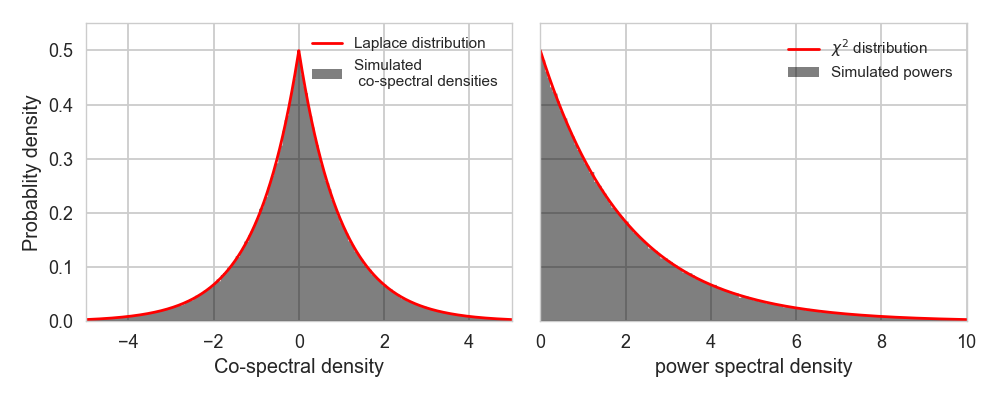
\includegraphics[width=\textwidth]{../figs/cs_dist.png}
\caption{Distribution of Leahy-normalized cospectral densities (left) and power spectral densities (right), respectively, for the simulated data. In dark grey, we show fine-grained histograms of the simulated powers. In red we plot the theoretical probability distribution the simulated powers should follow: A Laplace distribution with $\mu=0$ and $\sigma=2$ for the cospectral densities and a $\chi^2$-distribution with $2$ degrees of freedom for the power spectral densities. The simulated powers adhere very closely to the theoretical predictions.}
\label{fig:csdist}
\end{center}
\end{figure*}

\noindent where $K_0(x) = \int_{0}^{+\infty}{\frac{\cos{(xt)}}{\sqrt{t^2 + 1}} dt}$ is the Bessel function of the second kind of order $0$. We can now use this result to derive the probability density function of $C_j$. In particular, we find that both random variables $Z_j = A_{xj} A_{yj}$ and $Q_j = B_{xj} B_{yj}$ follow the Bessel distribution defined in Equation \ref{eqn:bessel}. Our task is therefore to find the PDF of the sum of two Bessel distributions. The PDF of this sum requires the convolution of the PDFs of each individual random variable being summed. This convolution is difficult to calculate directly for the Bessel distribution defined in Equation \ref{eqn:csdist} above. We instead consider the \textit{moment-generating function} of the PDF, generally defined as 

\begin{equation}
M_Z(t) := \mathbb{E}[e^{tZ}] \, 
\end{equation}

\noindent for a random variable $Z$. Consider the sum of any two independent random variables, $S = Z + Q$. While the PDF of $S$ can be found via the convolution of the individual PDFs, it is often simpler to consider the moment-generating function, where the convolution reduces to a simple multiplication operation:

\begin{equation}
M_S(t) = M_Z(t) M_Q(t) \, .
\end{equation} 

\noindent The moment-generating function of the Bessel distribution in Equation \ref{eqn:bessel} above is, in the general case \citep{seijas2012} where the means $\mu_x$ and $\mu_y$ are non-zero and the random variables may have unequal variances $\sigma_x \neq \sigma_y$: 

\begin{equation}
M_Z(t) = \frac{\exp{\left( \frac{t\mu_x \mu_y + 0.5 (\mu_y^2 \sigma_x^2 + \mu_x^2 \sigma_y^2) t}{1 - t^2 \sigma_x^2 \sigma_y^2} \right)}}{\sqrt{1 - t^2 \sigma_x^2 \sigma_y^2}}\, ,
\end{equation}
but since $\mu_x = \mu_y = 0$ for Fourier amplitudes, this reduces to
\begin{equation}
M_Z(t) =  \frac{1}{\sqrt{1 - t^2 \sigma_x^2 \sigma_y^2}}  \label{eqn:mgf},
\end{equation}

Thus, the moment-generating function for the sum of $Z_j$ and $Q_j$ becomes

\begin{equation}
M_C(t) = M_Z(t) M_Q(t) = \frac{1}{1 - t^2 \sigma_x^2 \sigma_y^2} \, .
\label{eqn:mgt_c}
\end{equation}

\noindent We note that the Laplace distribution is defined as 

\[
p_{\mathrm{Laplace}}(x | \mu, b) = \frac{1}{2b} \exp{\left(-\frac{|x - \mu|}{b} \right)}
\]

\noindent and its moment-generating function as

\[
M_\mathrm{Laplace}(t) = \frac{e^{t\mu}}{1 - b^2 t^2} \, .
\]

Comparing this last equation with Equation \ref{eqn:mgt_c}, we find that that Equation \ref{eqn:mgt_c} is equal to the moment-generating function of the Laplace distribution with $\mu = 0$ and $b = \sigma_x \sigma_y$, and hence the cospectral densities follow a Laplace distribution:

\begin{equation}
p(C_j | 0, \sigma_x\sigma_y) = \frac{1}{\sigma_x \sigma_y} \exp{\left(- \frac{|C_j|}{\sigma_x\sigma_y} \right)} 
\label{eqn:laplace}
\end{equation}

\noindent with

\begin{equation}
\sigma_x =  \sqrt{\frac{\sum_{k=1}^{N}{x_k}}{2}} \;\;\; \mathrm{and} \;\;\; \sigma_y =  \sqrt{\frac{\sum_{k=1}^{N}{y_k}}{2}} \, .
\label{eqn:csdist}
\end{equation}


\subsubsection{Detection Thresholds}
\label{sec:detectionthresholds}

Detection thresholds for cospectra will generally be different from those of classical power spectra, because the Laplace distribution tends to be narrower than the equivalent $\chi^2_2$ distribution for single power spectra. To show how the distributions and the corresponding detection thresholds differ, we simulated simple Poisson-distributed light curves. First, we simulated two light curves with a duration of $10\,\mathrm{s}$ and $10^6$ data points each, corresponding to a time resolution of $10^{-5}\,\mathrm{s}$. The light curves have an identical mean count rate of $10^{6} \, \mathrm{counts/s}$, corresponding to $10$ counts per bin. In order to simulate typical measurement uncertainties, we sampled from a Poisson distribution for each time bin with a rate parameter $\lambda = 10$, corresponding to the average counts per bin.

We then calculated both the cospectrum of the two light curves and the periodogram of only the first light curve for comparison. For simplicity, both spectra were computed in Leahy normalization \citep{leahy1983}, which is typically used when searching for (quasi-)periodic signals in time series.
In order to normalize the cospectrum correctly, we used $2/\sqrt{N_{\mathrm{ph}, x}N_{\mathrm{ph}, y}}$, where $N_{\mathrm{ph}, x}$ and $N_{\mathrm{ph}, y}$ are the number of photons of light curves $\mathbf{x}$ and $\mathbf{y}$, respectively, as prescribed by \citet{Bachetti+15}.
In this normalization the powers are distributed as $\chi^2_2$ exactly for the periodogram, and following a Laplace distribution with $\mu=0$ and $\sigma = 1$ for the cospectrum. In Figure \ref{fig:csdist}, we plot the resulting distribution of powers. While the periodogram is only defined for positive values, the Laplace distribution is symmetric around zero, and in general the cospectrum will comprise both positive and negative powers. It is also immediately visible from Figure \ref{fig:csdist} that the probability of obtaining a certain (positive) noise power is always lower for the Laplace distribution than for the $\chi^2$ distribution. In practice, this implies that using the latter where the former is appropriate, we may miss significant periodic signals, because we assume them to be weaker than they are in reality. To demonstrate this, we plot the survival function in Figure \ref{fig:survival}. The survival function, defined in terms of the CDF as $SF(x) = 1 - CDF(x)$, encodes the tail probability of seeing at least a value $x \geq X$. This tail probability is often considered to be the $p$-value of rejecting the null hypothesis that a certain candidate for a periodic signal could be reasonably produced by the noise powers. The CDF for the Laplace distribution with $\mu=0$ is defined as 

\begin{equation}
\label{eqn:cospectrum_cdf}
F_{C_j}(x)) = 
  \begin{cases} 
   \frac{1}{2} \exp{\left(\frac{C_j}{\sigma_x \sigma_y}\right)}  & \text{if } C_j < 0 \\
    1 - \frac{1}{2} \exp{-\left( \frac{C_j}{\sigma_x \sigma_y} \right)}   & \text{if } C_j \geq 0
  \end{cases}
\end{equation}

\noindent Much like the PDF, the tail probability is always smaller for the Laplace distribution, indicating that for a given candidate signal, the $p$-value for rejecting the null hypothesis will be stronger than for $\chi^2$-distributed variables. To reinforce this statement, we again simulated two light curves, each again with a duration of $10\,\mathrm{s}$, but this time with only $1000$ data points for simplicity and speed, and a time resolution of $0.01\,\mathrm{s}$. For this simulation, we assumed a mean count rate of $1000\,\mathrm{counts/s}$ or $10$ counts per bin, and additionally introduced a sinusoidal signal with a period of $0.1\,\mathrm{s}$ and a fractional rms amplitude of $a_\mathrm{frac} = 0.055$. Again, this template was used to produce two Poisson-distributed light curves with a rate parameter equal to the number of counts in each bin as defined by the flat continuum and the periodic signal. In Figure \ref{fig:cs_sim}, we show the cospectral densities along with trial-corrected $0.99$ detection thresholds for both the Laplace and $\chi^2$ distribution. If the powers are assumed to follow a $\chi^2$ distribution, as for the periodogram, the candidate at $10 \,\mathrm{Hz}$ would be discounted at the $99\%$ detection threshold, whereas correctly applying the Laplace distribution yields a correct rejection of the null hypothesis at the same detection threshold.

\begin{figure}
\begin{center}
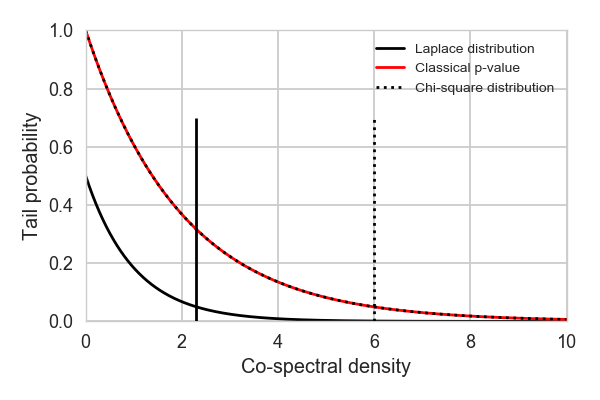
\includegraphics[width=9cm]{../figs/tailprob.png}
\caption{Tail probabilities for the Laplace and $\chi^2$ distributions, respectively. The tail probability, or survival function, is defined as $SF(x) = 1 - CDF(x)$. The tail probability measures the probability of observing a value $x\geq X$, and is often used for detecting periods in power spectra. For the power spectral densities, we plot both the theoretical prediction for the survival function based on the $\chi^2$ distribution (black dashed line), as well as the corrected distribution for power spectra derived in \citet{groth1975} (red solid line). For illustrative purposes, we show a single-trial $95\%$ detection threshold for the Laplace distribution (black solid vertical line) and the $\chi^2$ distribution (black dashed vertical line).}
\label{fig:survival}
\end{center}
\end{figure}

\begin{figure}
\begin{center}
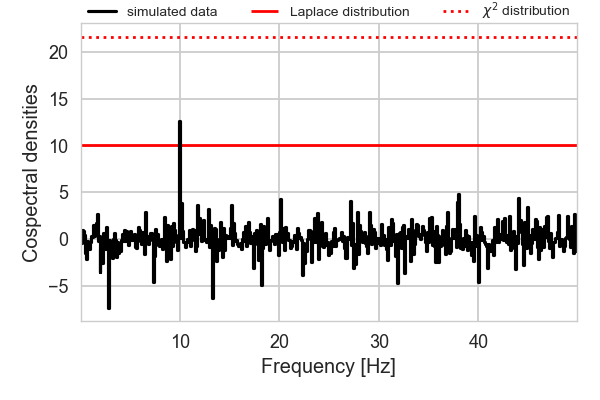
\includegraphics[width=9cm]{../figs/cs_detec.png}
\caption{Cospectrum of two simulated light curves, each with a constant continuum flux of $10$ counts per bin and a periodic signal at $10\,\mathrm{Hz}$. The latter is clearly visible in the cospectrum. We also show the 99\% detection threshold, corrected for a number of trials equal to the number of spectral bins, assuming Laplace-distributed data (red solid line) and $\chi^2$-distributed data (red dashed line). When the latter distribution is assumed, the periodic signal would not be considered a significant detection, because the $\chi^2$ distribution produces a wider distribution of powers. Applying the correct Laplace distribution, however, allows for the detection of weaker signals.}
\label{fig:cs_sim}
\end{center}
\end{figure}


\begin{figure*}
\begin{center}
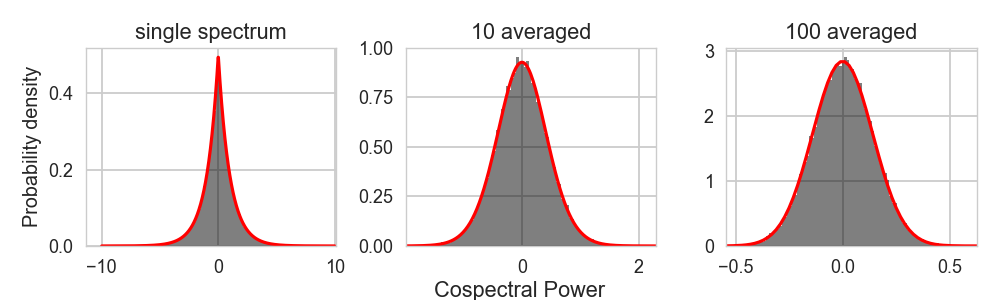
\includegraphics[width=\textwidth]{../figs/avg_dist.png}
\caption{Histogram of cospectral powers (grey) and the theoretical expectation (red) for three different cases. In the right panel, we show the distribution of powers for a single cospectrum, with its expected Laplace distribution from Equation \ref{eqn:laplace}, in the middle and right panel cospectral powers for averaging 10 (middle) and 100 (right) individual cospectra together. In the middle panel, the theoretical expectation of the sampling distribution is given by Equation \ref{eqn:averaged_pdf}, in the right panel by a Gaussian distribution with $\sigma=\sqrt{2/101}$.}
\label{fig:avg_dist}
\end{center}
\end{figure*}


\subsection{Averaged Cospectra}
\label{sec:averaged_cospectra}

The $\chi^2$ distribution used for periodograms has the simple property that sums of $\chi^2$-distributed variables again follow the same distribution, with a different number of degrees of freedom. The same is not true for the Laplace distribution. For $n$ independent and identically distributed (i.i.d.) random variables distributed following a standard Laplace distribution with a mean of $\mu = 0$ and a width of $b = 1$, the distribution of the sums of these random variables can be derived using the fact that a single Laplace random variable $X$ can be rewritten as the difference of two exponential random variables, 

\[
X = Z - Z' \; ,
\]
\noindent and thus for $n$ summed random Laplace random variables,

\begin{equation}
T = \sum_{i=1}^{n} X_i = \sum_{i=1}^{n}Z_i - \sum_{i=1}^{n} Z'_i = G_1 - G_2 \, ,
\end{equation}

\noindent where $G1$ and $G2$ are i.i.d.\ standard gamma random variables with a distribution $g(x) = \frac{1}{\Gamma(\nu)} x^{\nu-1} e^{-x}$ and a shape parameter $\nu = n$. For the full derivation of the density, we refer the reader to \citet{kotz2001} and simply state the end result for the PDF for $n$ averaged standard Laplace random variables, $\overline{X}_n$ (see \citealt{kotz2001}, Equations 2.3.25 and 2.3.26):

\begin{equation}
f_{\overline{X}_n}(x) = \frac{n e^{-|nx|}}{(n-1)! 2^n} \sum_{j=0}^{n-1} \frac{(n-1+j)!}{(n-1-j)! j!} \frac{|nx|^{n-1-j}}{2^j} \; \;\;, x \in R \; .
\label{eqn:averaged_pdf}
\end{equation}

For practical purposes, evaluating this PDF for averaged spectra above $n\sim 85$ is difficult numerically, because the factorials and exponents in the sum become very large and small, respectively. However, as we will show in Section \ref{sec:averaged_detthres} below, we find that in practice, when $n \gtrsim 30$, detection thresholds derived from Equation \ref{eqn:averaged_pdf} provide only a negligible difference over that derived from a normal distribution $N(0, \sqrt{2/(n+1)}$, depending on the significance threshold required and the number of trials. 

In order to derive tail probabilities useful for hypothesis testing, we require the CDF rather than the PDF. In order to correctly account for the absolute values in the PDF, we split the CDF into two parts: a case where $x < 0$ and a case where $x \geq 0$. The integral $F_{\overline{X}_n}(x) = P ( X \leq x) = \int_{\infty}^{x} f_{\overline{X}_n}(t) dt$ then becomes:

\begin{equation}
\label{eqn:averaged_cdf}
F_{\overline{X}_n}(x)) = 
  \begin{cases} 
   \sum_{j=0}^{n-1} D \frac{1}{n}(2\Gamma(-j+n) - \gamma(-j+n, nx)) \;, \;x \geq 0 \\
     \sum_{j=0}^{n-1} D  \frac{1}{n}\gamma(-j+n, -nx) \;,\; x < 0
  \end{cases}
\end{equation}

\noindent where $\Gamma(l)= (l-1)!$ is the gamma function, $\gamma(l+1, m) = l\gamma(l,m) - l^m e^{-m}$ is the incomplete upper gamma function, and the pre-factor constant $D$ is defined as 

\[
D = \frac{n(n-1+j)!}{(n-1-j)! (n-1)! 2^{n+j}} \, .
\]

\noindent As laid out in Section \ref{sec:detectionthresholds}, the tail probability can easily be calculated via the survival function, $\mathrm{SF}(x) = 1 - \mathrm{CDF}(x)$. 


\begin{figure*}
\begin{center}
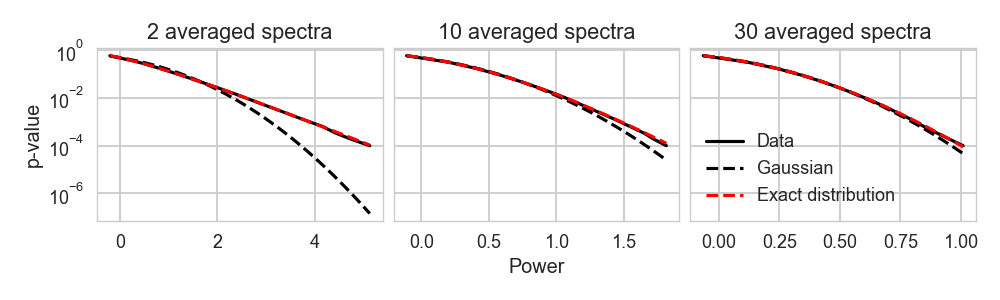
\includegraphics[width=\textwidth]{../figs/avg_pvalues.png}
\caption{Predictions for single-trial $p$-values as a function of cospectral power, for the simulated data sets (black solid line) compared to the theoretically predicted $p$-values using the CDF derived in Equation \ref{eqn:averaged_cdf} (red dashed line) as well as the survival function of a Gaussian distribution (black dashed line). The exact distribution matches the empirically derived tail probabilities from simulations within the uncertainties of the simulations. For the case of two averaged cospectra (left panel), a Gaussian approximation is obviously the wrong choice, and will lead to vastly overestimated significances, because the Gaussian PDF drops off much more sharply than the exact distribution. However, as more cospectra are averaged, the resulting distribution becomes more and more similar to that of a Gaussian (middle panel), and for $\sim$30 averaged cospectra, a Gaussian survival function yields a reasonably good approximation to the tail probabilities one would derive from simulations (right panel), up to $p \approx 10^{-4}$.}
\label{fig:avg_pvalue}
\end{center}
\end{figure*}

\subsubsection{Detection Thresholds}
\label{sec:averaged_detthres}

In order to show the way the probability distribution changes as a function of averaged cospectra, we simulate light curves of $10^{5}$ data points and a mean count rate of $100\,\mathrm{counts}/\mathrm{s}$ consisting of pure white noise. We compute $n$ such light curves and average their cospectral powers in order to show the distribution of those powers compared to the expected probability distributions. In Figure \ref{fig:avg_dist}, we show the simulated distribution of Leahy-normalized powers, along with the distributions that describe them. For a single, non-averaged spectrum, we use the Laplace PDF described in Equation \ref{eqn:laplace}. When averaging $10$ cospectra, we use Equation \ref{eqn:averaged_pdf} and show that the theoretical predictions agree with the simulated powers. Finally, for an averaged cospectra consisting of 100 individual light curves, Equation \ref{eqn:averaged_pdf} becomes difficult to compute numerically, and we use a Gaussian PDF instead, which describes the distribution of simulated powers well. 

In order to assess the effect on the $p$-values derived from averaged cospectra, we calculate the tail probabilities for the simulated data sets and compare them with the theoretically expected survival function as defined in Equation \ref{eqn:averaged_cdf} as well as a simple Gaussian distribution (Figure \ref{fig:avg_pvalue}). Similar to the results derived by \citet{balakrishnan1986}, we find that for cospectra of more than 30 averaged light curves, a Gaussian distribution yields a reasonably good approximation to the true distribution up to $p \approx 10^{-4}$ with lower overhead. Note, however, that this holds for single-trial probabilities. In general, one will wish to correct for calculating the significance of multiple trial frequencies, requiring the use of more stringent significance threshold. As shown in Figure \ref{fig:avg_pvalue}, the tail probabilities diverge as a function of power, and thus the Gaussian approximation will increasingly overestimate the significance of the signal the higher the threshold is set. Depending on the number of trials used, it is hence advisable to use Equation \ref{eqn:averaged_cdf} as long as it remains numerically stable (depending on implementation, up to $\sim$85 averaged cospectra).


\section{Example: A QPO in \nustar}
\label{sec:nustarqpo}

\begin{figure*}
\begin{center}
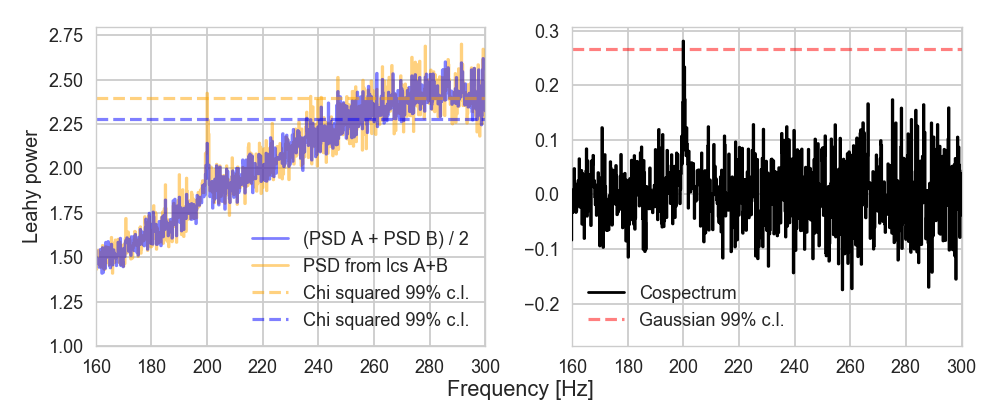
\includegraphics[width=\textwidth]{../figs/qpo.png}
\caption{Comparison of the averaged periodograms from the two detectors (blue), the periodogram obtained by the sum of the light curves (yellow; both left panel) and the cospectrum (right panel), for $3000\,\mathrm{s}$ of synthetic \nustar data with an incident count rate of $200 \mathrm{counts}\mathrm{s}^{-1}$ and a strong QPO at $200\,\mathrm{Hz}$. 
The QPO has an rms of $\sim$9\% and a high Q factor of $\sim$40. The shape of the periodogram is strongly distorted from the expected flat powerspectrum centred on a constant value of $2$, with deviations of more that $0.5$ in the mean level of the powers common. In dashed lines, we also show the expected (trial-corrected) $99\%$ confidence level for the periodograms (in the same colour, left panel) as well as the cospectrum (red, right panel). The signal is detected in both the periodogram of the combined light curves as well as the cospectrum. However, because the white noise level is variable in the periodogram and the power spectrum dips below the expected level of $2$ around the frequency of the QPO, the signal is not detected as significantly as it should have been if no dead time was present. Assessing the significance is much more straightforward in the cospectrum, which retains a flat baseline.
}
\label{fig:qpo}
\end{center}
\end{figure*}


In order to show the difference of the detection limits with the cospectrum and the power spectrum, we show how a QPO at 200 Hz from a very bright source would appear in \nustar. We simulate a light curve of $T=3000\mathrm{s}$ duration with a time resolution of $\delta t = 0.5 \,\mathrm{ms}$ and an average count rate of $200 \,\mathrm{counts}\,\mathrm{s}^{-1}$. To this constant background we add a quasi-periodic oscillation with a period of $5\,\mathrm{ms}$, a fractional rms amplitude of $f_\mathrm{rms} = 0.15$ and phases randomized using a normal distribution with a mean of $0$ and a width of $\sigma_\mathrm{qpo} = 0.01$. We then simulated photon events using rejection sampling from this light curve using the software package \textit{stingray}\footnote{\url{https://github.com/StingraySoftware/stingray}}, running the function \texttt{stingray.Eventlist.simulate\_times()} twice in order to produce two light curves that are statistically independent, but have the same signal and properties, as we would expect from an instrument with two independent detectors observing the same object. Subsequently we simulated variable deadtime for both light curves with an average time scale of $2.5 \,\mathrm{ms}$ as commonly seen in \nustar\ data \citep{Bachetti+15} using \textit{HENDRICS}\footnote{\url{https://github.com/StingraySoftware/HENDRICS}} \citep{bachetti2015b}. We then produced the periodogram of the summed light curves, the averaged periodogram of the two individual light curves, and the cospectrum of the two light curves. Note that in all three cases we produced averaged periodograms and co-spectra by splitting the light curves into 600 segments of $5\,\mathrm{s}$ length each in order to suppress the variance in the powers and show the effects of dead time more clearly.

The results are shown in Figure~\ref{fig:qpo}. While in all three cases, the QPO is clearly visible, the two periodograms show strong deviations from the expected flat power spectrum. The shape is distorted and requires a precise model of the non-linearly increasing baseline with a non-linearly increasing rms. While in principle, the periodogram of the combined light curves would have a higher significance by a factor of $\sqrt{2}$, the modeling requirements complicate the calculation of the significance of the QPO. 
The baseline of the cospectrum, conversely, is not distorted by dead time, and requires only an estimate of the \textit{local} rms in order to calculate the significance of the QPO using Equation~\ref{eqn:averaged_cdf}: it is sufficient to \textit{multiply the cospectrum around the feature by an estimate of the local standard deviation of the white noise} (which is 1 in the ideal case) to use the equations above with no modifications.

\section{Discussion and Conclusions}
\label{sec:discussion}
We have derived the statistical distribution for the cospectrum, defined as the real part of the cross spectrum. We show that because the Fourier amplitudes being multiplied to derive the cospectrum are now no longer identical (as is the case in the periodogram), the statistical distributions no longer reduce to a simple $\chi^2$ distribution with two degrees of freedom. Instead, we find that the powers in a single cospectrum follow a Laplace distribution with a mean of $\mu=0$ and a width of $\sigma=1$. This has important consequences for period detection. Most importantly, the Laplace distribution is considerably narrower than the $\chi^2_2$ distribution expected for periodograms, and thus the significance of a candidate periodic signal will generally be underestimated when using the latter. Using the correct distribution therefore helps correctly identifying weak signals, which the $\chi^2_2$ distribution would ignore as false negatives. 
Similarly, we find that the sums of Laplace distributions do not follow a similarly simple expression as in the periodogram case, but is considerably more computationally expensive, and may be difficult to estimate numerically when the number $n$ of averaged light curves in the final cospectrum is large. However, we find that for $n \gtrsim 30$, the statistical distribution can be well approximated by a Gaussian distribution, and the resulting tail probabilities used for period detection are very nearly the same as those derived from the exact distribution, up to a tail probability of $p \approx 10^{-4}$. This conclusion, however, depends sensitively on the detection threshold as well as the number of trials: for very small tail probabilities, the two distributions may still deviate significantly. For practical purposes, we suggest using Equation \ref{eqn:averaged_cdf} for at least up to $\sim$30 averaged cospectra, but also for averages of more spectra if significance thresholds for tail probabilities are smaller than $10^{-4}$, or the number of trials is large. 

As an example, we have simulated how a QPO would appear in \nustar\ in the presence of dead time, and have shown that the shape of the periodogram is strongly distorted, whereas that of the cospectrum is not (for a longer introduction into the cospectrum and how it can be used in the presence of dead time, see also \citealt{Bachetti+15}). The significance of the QPO is difficult to assess in the periodogram, because of the non-linearities introduced into the power spectrum by the variable dead time. The standard $\chi^2_2$ distributions may either overestimate or underestimate the significance, depending on the shape of the power spectrum at a given frequency, adding complexity to the detection process in the form of finding a non-linear model for the dead time. The cospectrum, on the other hand, only requires an estimate of the local variance in order to use the equations derived above, making it a far more convenient choice for periodicity detection.

The distributions laid out above allow for detecting periodic and narrow quasi-periodic signals in the presence of detector white noise, and especially important in the context of pulsar detection in X-rays, where faint sources may yield marginal detections even in the best of cases. At the same time, as instruments like \astrosat\ and \ixpe\ allow for observations with higher sensitivity, incorporating an accurate treatment of instrumental biases becomes increasingly important, and the cospectral statistics laid out here provide powerful tools to do so.
Notably absent from this discussion, however, is the much more common case where a source exhibits stochastic variability in the form of red noise or notably broadened quasi-periodic oscillations. In this case, the goal is either estimation of the precise properties of the underlying stochastic process, or detection of periods against a background varying stochastically. As has been shown above, the fact that the cross spectrum consists of two different time series complicates the statistical distributions considerably, and this is similarly true cospectra with variability. The exact treatment of this case is beyond the scope of this paper, and will be considered in depth in a forthcoming publication. 


\paragraph{Acknowledgements}
The authors thank Thomas Laetsch for helpful suggestions regarding the mathematical derivations.
Daniela Huppenkothen is supported by the James Arthur Postdoctoral Fellowship and the Moore-Sloan Data Science Environment at New York University. 
MB is supported in part by the Italian Space Agency through agreement ASI-INAF n.2017-12-H.0 and ASI-INFN agreement n.2017-13-H.0.


%%%%%%%%%%%%%%%%%%%%%%%%%%%%%%%%%%%%%%%%%%%%%%%%%%

%%%%%%%%%%%%%%%%%%%% REFERENCES %%%%%%%%%%%%%%%%%%

% The best way to enter references is to use BibTeX:
\bibliography{cospectra-paper}
\bibliographystyle{apj}

%%%%%%%%%%%%%%%%% APPENDICES %%%%%%%%%%%%%%%%%%%%%

\end{document}
